\documentclass[tikz]{standalone}
\usepackage[english]{babel}
\usepackage[T1]{fontenc}
\usepackage[utf8]{inputenc}
\usepackage[absolute,overlay]{textpos}
\usepackage{graphicx}
\usepackage[export]{adjustbox}
\usepackage{svg}
\usepackage{IEEEtrantools}
\usepackage{physics,dsfont,mathrsfs,cancel,tensor,slashed,mathtools}

\usepackage{amsmath}
\usepackage{amsfonts}
\usepackage{bm}
\usepackage{setspace}
\usepackage{subcaption}
\usepackage{mwe}
\usepackage{pgfplots}

\usepackage{tikz}
\usetikzlibrary{calc,patterns,decorations.pathmorphing,decorations.markings, angles, quotes}
\usetikzlibrary{arrows.meta}
\usetikzlibrary{decorations.pathreplacing}
\usepackage{tikzscale}

% ----------------------------
% Définition des nouvelles options xmin, xmax, ymin, ymax
% Valeurs par défaut : -3, 3, -3, 3
\tikzset{
xmin/.store in=\xmin, xmin/.default=-3, xmin=-3,
xmax/.store in=\xmax, xmax/.default=3, xmax=3,
ymin/.store in=\ymin, ymin/.default=-3, ymin=-3,
ymax/.store in=\ymax, ymax/.default=3, ymax=3,
}
% Commande qui trace la grille entre (xmin,ymin) et (xmax,ymax)
\newcommand {\grille}
{\draw[help lines] (\xmin,\ymin) grid (\xmax,\ymax);}
% Commande \axes
\newcommand {\axes} {
\draw [>=stealth,->] (\xmin,0) -- (\xmax,0);
\draw [>=stealth,->] (0,\ymin) -- (0,\ymax);
}
% Commande qui limite l’affichage à (xmin,ymin) et (xmax,ymax)
\newcommand {\fenetre}
{\clip (\xmin,\ymin) rectangle (\xmax,\ymax);}
% ----------------------------

\begin{document}


    
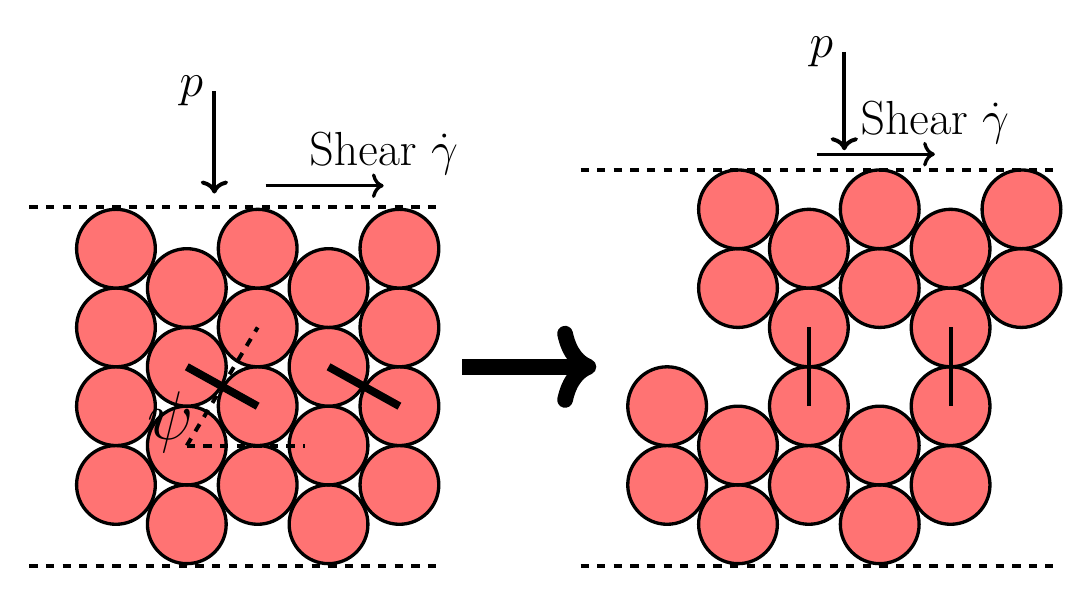
\begin{tikzpicture}[scale = 1.]
    % \draw (-11.5,4) node {\textbf{A}};
    % \draw (-1.5,4) node {\textbf{B}};

    \def \b {7};
    \def \c {-7};
    \def \d {0.1};
    \def \r {0.5};

    % Before dilatancy
    \foreach \x in {1.1, 2.9, 4.7}
        \foreach \y in {1.5,..., 4.5}
            \draw [color=black, fill=red!55,very thick] (\x, \y) circle (0.5);

    \foreach \x in {2, 3.8}
        \foreach \y in {1,..., 4}
            \draw [color=black, fill=red!55,very thick] (\x, \y) circle (0.5);

    %contact forces
    \draw[ very thick, line width = 1mm] (2.9, 2.5) -- (2,3);
    \draw[ very thick,line width = 1mm] (4.7, 2.5) -- (3.8,3);
    
    \draw[dashed, very thick] (0, 5.03) -- (5.2,5.03);
    \draw[dashed, very thick] (0, 0.47) -- (5.2,0.47);

    % \draw[->, very thick, line width = 1mm]  (0.1, 4.2) node[left] {\LARGE $p$} -- (0.1, 5.03) ;
     
    \draw [very thick, ->] (3, 5.3) -- (4.5, 5.3) node[above] {\LARGE Shear $\dot\gamma$};

        \draw[->, very thick, line width = 0.5mm]  (2.35, 6.5) node[left] {\LARGE $p$} -- (2.35, 5.2) ;

    \draw[->, line width = 2mm] (5.5, 3) -- (7.2,3);
    
    %When dilatating
    
    \foreach \x in {1.1, 2.9, 4.7}
        \foreach \y in {1.5,2.5}
            \draw [color=black, fill=red!55,very thick] (\x+\b, \y) circle (0.5);

    \foreach \x in {2, 3.8}
        \foreach \y in {1,2}
            \draw [color=black, fill=red!55,very thick] (\x+\b, \y) circle (0.5);

    \foreach \x in {2.9, 4.7}
        \foreach \y in {3.5, 4.5}
            \draw [color=black, fill=red!55,very thick] (\x+\b, \y) circle (0.5);

    \foreach \x in {2, 3.8, 5.6}
        \foreach \y in { 4,5}
            \draw [color=black, fill=red!55,very thick] (\x+\b, \y) circle (0.5);

    \draw[dashed, very thick] (0+\b, 0.47) -- (6+\b,0.47);
    \draw[dashed, very thick] (0+\b, 5.5) -- (6+\b,5.5);


    \draw[->, very thick, line width = 0.5mm]  (3.35+\b, 7) node[left] {\LARGE $p$} -- (3.35+\b, 5.75) ;
     
    \draw [very thick, ->] (3+\b, 5.7) -- (4.5+\b, 5.7) node[above] {\LARGE Shear $\dot{\gamma}$};

    \draw[ very thick, line width = 0.5mm] (2.9+\b, 2.5) -- (2.9+\b,3.5);
    \draw[ very thick,line width = 0.5mm] (4.7+\b, 2.5) -- (4.7+\b,3.5);

    \coordinate (A) at (4, 2);
    \coordinate (B) at (2, 2);
    \coordinate (C) at (2.2, 2.4);
    \draw[dashed, thick, line width = 0.5mm] (2, 2) -- (3.5, 2);
    \draw[dashed, thick, line width = 0.5mm] (2, 2) -- (2.9, 3.5);
    \pic [draw, -,, angle eccentricity=1.5] {angle = A--B--C};
    
    \node[color = black] at (1.8, 2.3)  {\Huge $\psi $};
    % \node at (0, 6)  {\LARGE (a) $\psi > 0$};

\end{tikzpicture}


    
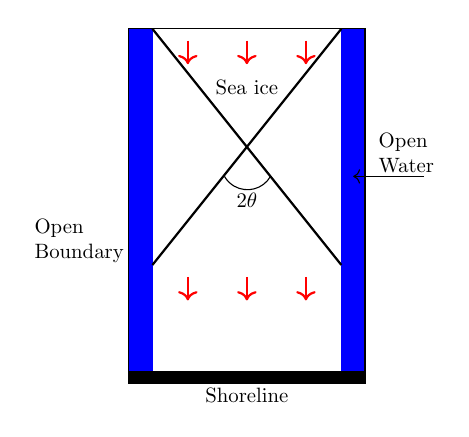
\begin{tikzpicture}[scale = 1.5]

   
    % \node at (1, -0.1) {\tiny Shoreline};

    \draw[->, thick, red] (0.5, 2.9) -- (0.5, 2.7);
    \draw[->, thick, red] (1, 2.9) -- (1, 2.7);
    \draw[->, thick, red] (1.5, 2.9) -- (1.5, 2.7);

    % \draw[->, thick, red] (0.5, 1.9) -- (0.5, 1.7);
    % \draw[->, thick, red] (1, 1.9) -- (1, 1.7);
    % \draw[->, thick, red] (1.5, 1.9) -- (1.5, 1.7);

    \draw[->, thick, red] (0.5, 0.9) -- (0.5, 0.7);
    \draw[->, thick, red] (1, 0.9) -- (1, 0.7);
    \draw[->, thick, red] (1.5, 0.9) -- (1.5, 0.7);

    
    \filldraw[blue] (0, 0) rectangle (0.2, 3);
    \filldraw[blue] (1.8, 0) rectangle (2, 3);
    \node[scale = 0.75] at (1, 2.5) { Sea ice};
    \node[scale = 0.75] at (1, -0.1) { Shoreline};
    \node[scale = 0.75, align = left] at (-0.42, 1.2) {Open \\ Boundary};
    \filldraw (0,0) rectangle (2,0.1);
    \draw (0,0) rectangle (2,3);

    
    \draw[->] (2.5, 1.75) -- (1.9, 1.75) ;
   \node[scale = 0.75, align = left] at (2.35, 1.95) {Open \\ Water};



    \draw[-, thick] (0.2, 3) -- (1.8, 1);
    \draw[-, thick] (0.2, 1) -- (1.8, 3);

    \draw  (1.2,1.75) arc[start angle = -30, end angle=-150,radius=0.225] ;
    \node[scale = 0.75] at (1, 1.55) {$2\theta$};
    
\end{tikzpicture}


    


\begin{tikzpicture}[scale = 4]
    % \draw (-11.5,4) node {\textbf{A}};
    % \draw (-1.5,4) node {\textbf{B}};


    \draw[thick, ->] (0, 0.2)--(0, 1.5) node[right] {$p$};

    \draw[thick,->] (-0.75, 1)--(0.75, 1)node[below] {$\dot{\epsilon}_\text{I}$};

    \draw[thick,-, red] (-0.75, 0.5)--(0, 0.5);
    \draw[thick,-, red] (0, 0.5)--(0, 1);
    \draw[thick,-, red] (0,1)--(0.75, 1);


    \draw[thick,dashed, blue] (-0.75, 0.5)--(0.2, 0.5);
    \draw[thick,dashed, blue] (0.2, 0.5)--(0.2, 1);
    \draw[thick,dashed, blue] (0.2,1)--(0.75, 1);

    \node at (-0.2, 0.4) {$P_{max}$};

    \draw [decorate,decoration={brace,amplitude=5pt,raise=0ex}]
  (0,1) -- (0.2,1) node[above]{$\nabla \cdot u = \dot \gamma \tan \psi$};

    
\end{tikzpicture}



    
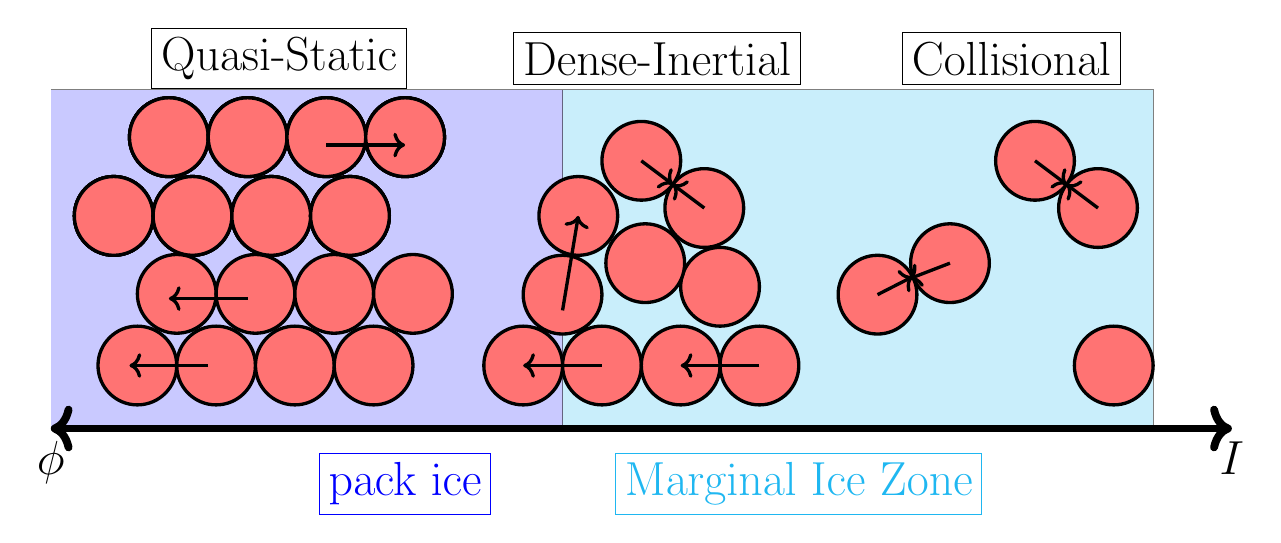
\begin{tikzpicture}[scale = 1]


    \def \b {0};
    \def \c {0.1};
    \def \d {0.1};
    \def \r {2.3};

    \draw[fill=blue!42, opacity = 0.5] (0,-0.5) -- (6.5, -0.5) -- (6.5,3.8) -- (0,3.8 );

    \draw[fill=cyan!42, opacity = 0.5] (6.5, -0.5) -- (14, -0.5) -- (14,3.8) -- (6.5,3.8 );

    \node[draw] at  (2.9, 4.2) { \LARGE Quasi-Static};
    % \node[draw] at (-4,2.7-3.7) { \LARGE Collision};

    \foreach \x in {1, ..., 4}
            \draw [color=black, fill=red!55,very thick] (\x + \b+0.1, 0.3) circle (0.5);

        \foreach \x in {1.5, ..., 4.5}
            \draw [color=black, fill=red!55, very thick] (\x + \b+0.1, 1.21) circle (0.5);

    \foreach \x in {1, ..., 4}
        \foreach \y in {1.5, ..., 4.5}
            \draw [color=black, fill=red!55,very thick] (\x + \b-0.2, 2.2) circle (0.5);


    \foreach \x in {1.5, ..., 4.5}
        \foreach \y in {1.5, ..., 4.5}
            \draw [color=black, fill=red!55,very thick] (\x + \b, 3.2) circle (0.5);

        

    \draw [very thick, ->] (3.5 + \b, 3.1) -- ( 3.5+ \b + 1 , 3.1);
    
    \draw [very thick, ->] (2.5 + \b, 1.15) -- ( 2.5+ \b -1  , 1.15);

    \draw [very thick, ->] (2. + \b, 0.3) -- ( 2.+ \b -1  , 0.3);


    \def \b {5};
    \def \c {0.1};
    \def \d {0.1};
    \def \r {2.3};


    \node[draw] at  (2.7+\b, 4.2) { \LARGE Dense-Inertial};
    % \node[draw] at (-4,2.7-3.7) { \LARGE Collision};

    \foreach \x in {1, ..., 4}
            \draw [color=black, fill=red!55,very thick] (\x + \b, 0.3) circle (0.5);

    % \foreach \x in {1.5, ..., 3.5}
    %         \draw [color=black, fill=red!55, very thick] (\x + \b, 1.3) circle (0.5);
            
    \draw [color=black, fill=red!55, very thick] (1.5 + \b, 1.2) circle (0.5);       
    \draw [color=black, fill=red!55, very thick] (3.5 + \b, 1.3) circle (0.5);  
    \draw [color=black, fill=red!55, very thick] (2.55 + \b, 1.6) circle (0.5);
    \draw [color=black, fill=red!55, very thick] (3.3 + \b, 2.3) circle (0.5);
    \draw [color=black, fill=red!55, very thick] (1.7 + \b, 2.2) circle (0.5);
    \draw [color=black, fill=red!55, very thick] (2.5 + \b, 2.9) circle (0.5);


        
    \draw [very thick, ->] (2.5 + \b, 2.9) -- (2.9 + \b, 2.6);
    \draw [very thick, ->] (3.3 + \b, 2.3) -- (2.9 + \b, 2.6);
    
   \draw [very thick, ->] (1.5 + \b, 1.) -- (1.7 + \b, 2.2);

    \draw [very thick, ->] (2. + \b, 0.3) -- ( 2.+ \b -1  , 0.3);
    \draw [very thick, ->] (4. + \b, 0.3) -- ( 4.+ \b -1  , 0.3);


    \def \b {10};
    \def \c {0.1};
    \def \d {0.1};
    \def \r {2.3};


    \node[draw] at  (2.2+\b, 4.2) { \LARGE Collisional};
            
    \draw [color=black, fill=red!55, very thick] (.5 + \b, 1.2) circle (0.5);    
    \draw [color=black, fill=red!55, very thick] (1.42 + \b, 1.6) circle (0.5);
    \draw [color=black, fill=red!55, very thick] (3.5 + \b, 0.3) circle (0.5);  
    \draw [color=black, fill=red!55, very thick] (3.3 + \b, 2.3) circle (0.5);
    \draw [color=black, fill=red!55, very thick] (2.5 + \b, 2.9) circle (0.5);


        
    \draw [very thick, ->] (2.5 + \b, 2.9) -- (2.9 + \b, 2.6);
    \draw [very thick, ->] (3.3 + \b, 2.3) -- (2.9 + \b, 2.6);

    \draw [very thick, ->] (.5 + \b, 1.2) -- (0.95 + \b, 1.43);
    \draw [very thick, ->] (1.42 + \b, 1.6) -- (0.9 + \b, 1.4);

    \draw [very thick, line width = 1mm, <->] (0 , -0.5) node[below] {\LARGE $\phi$} -- (15, -0.5) node[below] {\LARGE $I$};


    \node[draw, color = blue] at (4.5, -1.2) {\LARGE pack ice};


    \node[draw, color = cyan!88] at (9.5, -1.2) {\LARGE{Marginal Ice Zone}};
\end{tikzpicture}


    

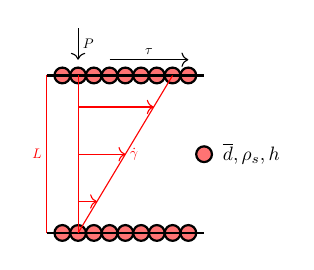
\begin{tikzpicture}[scale=2][font=\sffamily]
\foreach \x in { 0.1, 0.2,0.3, 0.4, 0.5,0.6, 0.7, 0.8, 0.9}
            \draw [color=black, fill=red!55, thick] (\x, 0) circle (0.05);

\foreach \x in { 0.1, 0.2,0.3, 0.4, 0.5,0.6, 0.7, 0.8, 0.9}
            \draw [color=black, fill=red!55, thick] (\x, 1) circle (0.05);


\draw [color=black, fill=red!55, thick] (1, 0.5) circle (0.05) node[scale = 0.7] at (1.3, 0.5){$\overline{d}, \rho_s, h$};

            
\draw[-, thick] (0, 1) -- (1, 1);

\draw[-, thick] (0, 0) -- (1, 0);



\draw[-, red] (0.2, 0) -- (0.2, 1);

\draw[-, red] (0.2, 0) -- (0.8, 1) node[midway, right, scale = 0.5] {$\Dot{\gamma}$};

\draw[->, red] (0.2, 0.2) -- (0.32, 0.2);
\draw[->, red] (0.2, 0.5) -- (0.5, 0.5);
\draw[->, red] (0.2, 0.8) -- (0.68, 0.8);

\draw[-, red] (0, 0) -- (0.0, 1) node[midway, left, scale = 0.5] {$L$}; 

\draw[->] (0.2, 1.3) -- (0.2, 1.1) node[midway, right, scale = 0.5] {$P$} ;

\draw[->] (0.4, 1.1) -- (0.9, 1.1) node[midway, above, scale = 0.5] {$\tau$};



\end{tikzpicture}


    
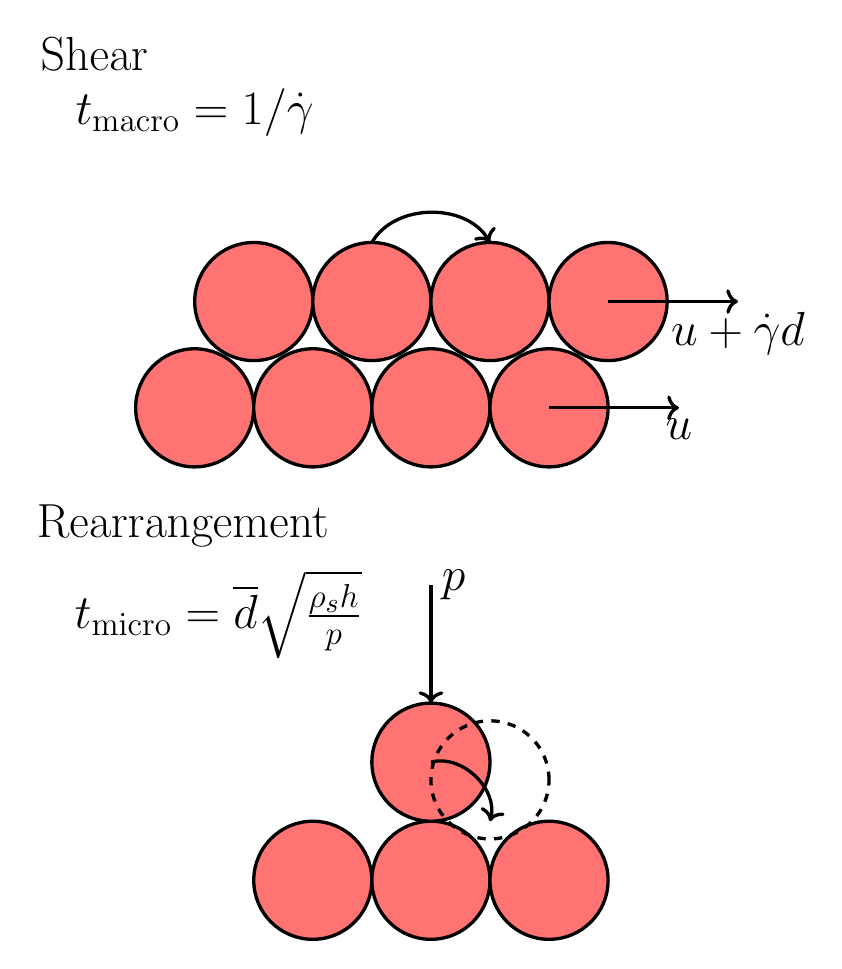
\begin{tikzpicture}[scale = 1.5]
    % \draw (-11.5,4) node {\textbf{A}};
    % \draw (-1.5,4) node {\textbf{B}};

    \def \b {4};
    \def \c {-7};
    \def \d {0.1};
    \def \r {0.5};
    \node at (1.15, 4)  {\LARGE Shear};
    \node at (2, 3.5)  {\LARGE $t_\text{macro} = 1/\dot{\gamma}$};

    % \node at (2, 3.5)  {\LARGE $v _\text{macro} = \overline{d} \dot{\gamma}$};
    % Before dilatancy
    \foreach \x in { 2, 3, 4, 5}
        \foreach \y in {1}
            \draw [color=black, fill=red!55,very thick] (\x, \y) circle (0.5);

    \foreach \x in { 2.5, 3.5, 4.5, 5.5}
        \foreach \y in {1.9}
            \draw [color=black, fill=red!55,very thick] (\x, \y) circle (0.5);
            
    \draw[->, very thick] (5, 1) -- (6.1, 1) node[below] {\LARGE $u$};
    \draw[->, very thick] (5.5, 1.9) -- (6.6, 1.9) node[below] {\LARGE $u + \dot{\gamma} d$};
    \draw[->, very thick, black] (3.5, 2.4) to [bend left=60] (4.5,2.4);

    \node at (1.9, 3.5-3.5)  {\LARGE Rearrangement};
    % Before dilatancy
    \foreach \x in { 3, 4, 5}
        \foreach \y in {1-\b}
            \draw [color=black, fill=red!55,very thick] (\x, \y) circle (0.5);

            \draw [color=black, fill=red!55,very thick] (4, 2-\b) circle (0.5);
            
    \draw [color=black,dashed,very thick] (4.5, 1.85-\b) circle (0.5);
    \draw[->, very thick, black] (4, 2-\b) to [bend left=60] (4.5,1.5-\b);
    \draw[->, very thick] (4, 3.5-\b) node[right] {\LARGE $p$}  -- (4, 2.5-\b) ;

    \node at (2.2, 2.75-3.5)  { \LARGE $t_\text{micro} = \overline{d}\sqrt{\frac{\rho_s h}{p}}$};
    
    
    % \node at (2.2, 2.75-3.5)  {\LARGE $v_\text{micro} = \sqrt{\frac{p}{\rho_s h}}$};


\end{tikzpicture}


    \documentclass[crop,tikz]{standalone}
\usepackage{tikz}
\usetikzlibrary{decorations.pathmorphing}
\begin{document}


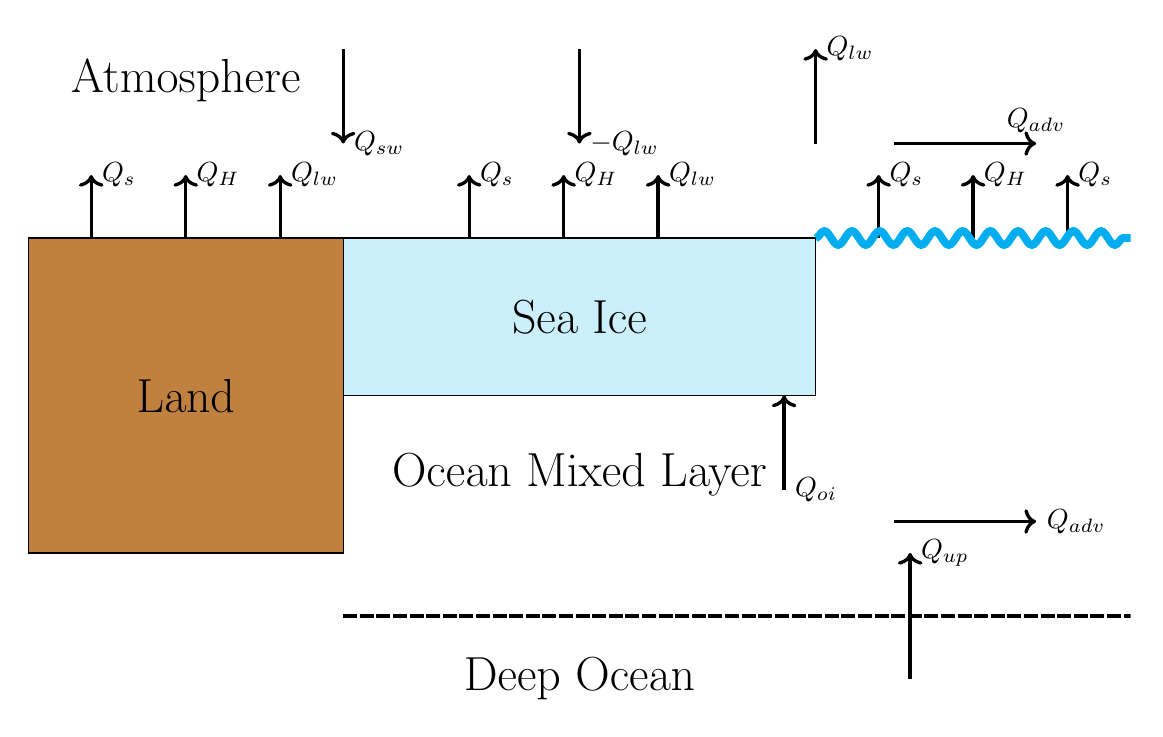
\begin{tikzpicture}[scale = 4]
\draw[fill=cyan!20] (1,0.5) rectangle (2.5,1); 
\draw[fill=brown] (0,0) rectangle (1,1); 

\draw[dashed, very thick] (1, -0.2) rectangle (3.5,-0.2); 

%---- Atmospheric fluxes
\draw[->, very thick] (0.2, 1) -- (0.2, 1.2) node[right] {$Q_s$};
\draw[->, very thick] (0.5, 1) -- (0.5, 1.2) node[right] {$Q_H$};
\draw[->, very thick] (0.8, 1) -- (0.8, 1.2)  node[right] {$Q_{lw}$};


\draw[->, very thick] (1.1+0.3, 1) -- (1.1+0.3, 1.2) node[right] {$Q_s$};
\draw[->, very thick] (1.4+0.3, 1) -- (1.4+0.3, 1.2) node[right] {$Q_H$};
\draw[->, very thick] (1.7+0.3, 1) -- (1.7+0.3, 1.2) node[right] {$Q_{lw}$};

\draw[->, very thick] (1.1+1.6, 1) -- (1.1+1.6, 1.2)node[right] {$Q_s$};
\draw[->, very thick] (1.4+1.6, 1) -- (1.4+1.6, 1.2)node[right] {$Q_H$};
\draw[->, very thick] (1.7+1.6, 1) -- (1.7+1.6, 1.2)node[right] {$Q_s$};


\draw[->, very thick] (1, 1.6) -- (1, 1.3)node[right] {$Q_{sw}$};
\draw[->, very thick] (1.75, 1.6) -- (1.75, 1.3) node[right] {$-Q_{lw}$};
\draw[->, very thick] (2.5, 1.3) -- (2.5, 1.6) node[right] {$Q_{lw}$};

\draw[->, very thick] (2.75, 1.3) -- (3.2, 1.3) node[above] {$Q_{adv}$};;

%--- Oceanic fluxes
\draw[->, very thick] (2.4, 0.2) node[right] {$Q_{oi}$} -- (2.4, 0.5);
\draw[->, very thick] (2.8, -0.4) -- (2.8, 0) node[right] {$Q_{up}$};
\draw[->, very thick] (2.75, 0.1) -- (3.2, 0.1) node[right] {$Q_{adv}$};
\draw[decorate,decoration=snake,cyan, line width = 1mm]  (2.5,1) - - (3.5,1) ;


\node at (0.5,0.5) {\LARGE Land};
\node at (1.75,0.75) {\LARGE Sea Ice};
\node at (1.75,0.25) {\LARGE Ocean Mixed Layer};
\node at (1.75,-0.4) {\LARGE Deep Ocean};
\node at (0.5,1.5) {\LARGE Atmosphere};




\end{tikzpicture}

\end{document}


\end{document}